\documentclass[prd,twocolumn,amsmath,amssymb,floatfix,superscriptaddress,nofootinbib]{revtex4-1}
\usepackage{bm}
\usepackage{amsmath}
\usepackage{epsfig}
\usepackage{color}
\usepackage{natbib}
\usepackage{textcase}
\usepackage{graphicx}
\usepackage{ifthen}
\usepackage{xstring}
\usepackage{graphicx}
\usepackage[utf8]{inputenc} 
\usepackage{amssymb}
\usepackage{latexsym}
\usepackage{epstopdf}
\epstopdfsetup{update}
\DeclareGraphicsExtensions{.ps, .png}
\epstopdfDeclareGraphicsRule{.ps}{pdf}{.pdf}{ps2pdf -dEPSCrop -dNOSAFER #1 \OutputFile} 
\usepackage{dcolumn} 
\usepackage{multirow}
\usepackage{appendix}
\usepackage{footnote}
\usepackage{tabularx,ragged2e,booktabs}
\usepackage[normalem]{ulem}
\usepackage{float}
\restylefloat{table}

\newcommand{\refsec}[1]{section~\ref{sec:#1}}
\newcommand{\refeq}[1]{Eq.~(\ref{eq:#1})}
\newcommand{\refssec}[1]{section~\ref{subsec:#1}}
\newcommand{\reffig}[1]{Fig.~\ref{fig:#1}}
\newcommand{\refFig}[1]{Fig.~\ref{fig:#1}}

\newcommand{\xef}{x_e^{\rm fid}}
\newcommand{\xmax}{x_e^{\rm max}}
\newcommand{\zmax}{z_{\rm max}}
\newcommand{\zmin}{z_{\rm min}}
\newcommand{\zre}{z_{\rm re}}
\newcommand{\xemin}{x_e^{\rm min}}
\newcommand{\lsc}{\mathcal{L}}
\newcommand{\tauhi}{\tau_{\rm hi}}
\newcommand{\taulo}{\tau_{\rm lo}}
\newcommand{\sample}{{\rm sample}}

\newcommand{\ra}{\rightarrow}
\def\max{_{\mathrm{max}}}
\def\lsim{\mathrel{\raise.3ex\hbox{$$<$$\kern-.75em\lower1ex\hbox{$\sim$}}}}
\def\gsim{\mathrel{\raise.3ex\hbox{$$>$$\kern-.75em\lower1ex\hbox{$\sim$}}}}

\newcommand{\beq}{\begin{equation}}
\newcommand{\eeq}{\end{equation}}

\newcommand{\bea}{\begin{eqnarray}}
\newcommand{\eea}{\end{eqnarray}}

\newcommand{\wh}[1]{\textcolor{blue}{#1}}
\newcommand{\ch}[1]{\textcolor{red}{#1}}

\def\mnras{Mon.\ Not.\ R.\ Astron.\ Soc.\ }
\definecolor{darkgreen}{cmyk}{0.85,0.2,1.00,0.2} 
\definecolor{purple}{cmyk}{0.5,1.0,0,0} 
\def\physrep{Phys.~Rep.}

\definecolor{ultramarine}{rgb}{0.07, 0.04, 0.56}
\definecolor{cadmiumgreen}{rgb}{0.0, 0.42, 0.24}
\definecolor{indigo(dye)}{rgb}{0.0, 0.25, 0.42}
\usepackage[linktocpage=true]{hyperref}
\hypersetup{
colorlinks=true,
citecolor=ultramarine,
linkcolor=cadmiumgreen,
urlcolor=indigo(dye),
pdfauthor={},
pdftitle={},
pdfsubject={}
}


\begin{document}
	
\title{Effective Reionization Likelihood from Planck 2018 Data (?)}

\author{Chen Heinrich}\email{chenhe@caltech.edu}
\affiliation{California Institute of Technology, Pasadena, California 91109, USA}
\affiliation{Jet Propulsion Laboratory, California Institute of Technology, Pasadena, California 91109, USA}

\author{Wayne Hu}
\affiliation{Kavli Institute for Cosmological Physics, Enrico Fermi Institute, University of Chicago, Chicago Illinois 60637}
\affiliation{Department of Astronomy \& Astrophysics,
 University of Chicago, Illinois 60637}

\begin{abstract}

...

\end{abstract}
\pacs{}

\maketitle




\section{Introduction}
\label{sec:intro}

The cosmic microwave background (CMB) has entered an era of precision cosmology. The measurements from the \textit{Planck} satellite have shown agreement with the standard $\Lambda$CDM model which describes the initial perturbations in the Universe and their evolution. While many components of the standard cosmology model is well-understood, the details of the process of reionization however, remains one of the most uncertain pieces. Its uncertainty propagates into the inferences of other important parameters such as the primordial power spectrum amplitude. Through it, the uncertainty in reionization will become one of the major sources of uncertainty for measuring the sum of neutrino masses from future gravitational lensing measurements of the CMB; and will also have implications for inferring cosmic acceleration through the growth of structure. [add more refs here]

Typically, the impact of reionization on the primary CMB fluctuations has been modeled as a steplike transition in the global ionization history, with the step location parameterized by the total Thomson optical depth induced. This steplike model describes a Universe in which all hydrogen becomes fully ionized almost instantaneously at one particular redshift, and assumes, by construction, that there is negligible ionization before the transition. However, through the shape of the reionization bump induced in the CMB E-mode polarization at large angles, more information on the coarse-grained evolution of the ionization history can be obtained. 

In fact, to extract the most information possible from this E-mode bump, Ref.~\cite{Hu:2003gh, Mortonson:2007hq} developed the principal component (PC) method, where a few PCs is sufficient to describe the entire model space of physical ionization histories regarding their observable impact on the large-angle $E$-mode power spectrum. This method has been applied to WMAP and Planck data to obtain complete constraints on reionization models~\cite{Mortonson:2008rx, Mortonson:2007hq, Heinrich:2016ojb, Aghanim:2018eyx}. It was also adopted for a Planck 2013 analysis for marginalizing ionization history when constraining inflationary parameters in Ref.~\cite{Planck:2013jfk}, as well as massive neutrinos and gravitational waves in Ref~\cite{Dai:2015dwa}[also cite our inflation papers?]. 

In a re-analysis of the Planck 2015 data with PCs~\cite{Heinrich:2016ojb}, a component of the high-redshift ionization that would have been missed by a simple steplike model~\cite{Heinrich:2016ojb} was uncovered. In the latest official Planck 2018 release~\cite{Aghanim:2018eyx}, the PC method was also adopted to probe ionization at high-redshift, whose significance was reduced since the Planck 2015 release, largely due to the reduction of systematics at large-scales~\cite{Aghanim:2018eyx, Heinrich:2018btc}. In addition to PCs, the FlexKnot method was employed, which is also able to capture general ionization histories by varying the number of ``knots" in redshifts and the amplitude of the ionization fraction at these knots. 
% Planck intermediate results on reionization history: \cite{Adam:2016hgk}

Since the release of the Planck 2018 official analysis, an improved likelihood for the low-$\ell$ $E$-mode polarization was publicly released in 2019. This new likelihood, called $\texttt{srollv2}$, allows for improved reionization constraints with its better foreground modeling: The error bar on the optical depth $\tau$ in the steplike model is reduced by roughly a factor of two from XX to XX. [fill in numbers]

Since the Planck final release will likely be the best full-sky survey from space available to us in the next decade, it is important to extract all the information present in the data. In light of the $\texttt{srollv2}$ likelihood release, we obtain new reionization PC constraints with this latest likelihood. Enabled by the completeness property of the PCs, we also turn these constraints into an effective likelihood useful for assessing the CMB likelihood of \textit{any} reionization model out to $\zmax$ = 30, following techniques tested in Ref.~\cite{Heinrich:2016ojb}. 

The code is publicly available on GitHub\footnote{[give link]}. [a bit more description here]. [comment on speed]. [comment on joint likelihood].

Extending PCs to cover up to $z_{\rm max} = 50$,we verified that there is no hint of ionization beyond $z>30$ in this Planck data release. But for the high-z ionization below $z=30$, we did find a less stringent constraint on $\tau(15, 30)$, the optical depth in the redshift range 15 to 30, that is XX times less stringent than the Planck official results using Flex Knots [fill in number and make sure to say its flex knot or PC] in Ref.~\cite{Aghanim:2018eyx}. Moreover, we demonstrate that the PC results of Ref.~\cite{Aghanim:2018eyx} suffers from a logical flaw in the treatment of its priors following Ref.
~\cite{Millea:2018bko} and ends up penalizing lower optical depth models. [quote difference in tau(15, 30) or total tau possibly attributed to this treatment]. %We follow the appendix of Ref.~\cite{Heinrich:2018btc} for the Planck 2015 data

The paper is structured as follows. We first describe in section~\ref{sec:background} the background on the reionization principal components and the kernel density estimate (KDE) technique used for building the effective likelihood. Then in section~\ref{sec:results}, we describe the PC results using the Planck 2018 + \texttt{srollv2} likelihood, and compare with previous results in literature. Then in section~\ref{sec:effective_likelihood}, we present the effective likelihood code, and demonstrate its fidelity with two examples, 1) the standard steplike model, and 2) a two-parameter model where a plateau of ionization at high-$z$ is added to the standard one-step model for illustration purposes. Finally, we summarize our results and conclude in section~\ref{sec:conclusion}.
\section{Background}
\label{sec:background}
The principal component technique for constraining reionization using the large-angle $C_\ell^{EE}$ polarization spectrum was first introduced in Ref.~\cite{Hu:2003gh}. We now briefly summarize the PC technique in section~\ref{sec:PC}, as well as the kernel density estimate technique for building the effective likelihood in section~\ref{sec:KDE}. We refer the readers to Refs.~\cite{Hu:2003gh, Mortonson:2008rx, Mortonson:2007hq, Heinrich:2018btc}[pick 1-2] and Refs.~\cite{Heinrich:2016ojb} respectively for a more complete description on these topics.
\subsection{Reionization Principal Components}
\label{sec:PC}
We begin by parametrizing $x_e(z)$, the ionization fraction relative to the fully ionized hydrogen at redshift $z$, into its principal components $S_{a}(z)$ with respect to the CMB $E$-mode polarization:
%
\begin{equation}
x_e(z)=\xef(z)+\sum_{a}m_{a}S_{a}(z),
\label{eq:mmutoxe}
\end{equation}
%
where $m_a$ are the PC amplitudes and $\xef(z)$ is the fiducial model. We obtain the PCs $S_{a}(z)$ as eigenfunctions of the Fisher information matrix for $x_e(z)$ in a given range $z_{\rm min}<z<z_{\rm max}$ from cosmic variance limited $C_\ell^{EE}$ measurements 
%
\beq
F_{ij} = \sum_l \frac{1}{\sigma_l^2} \frac{\partial C_l^{EE}}{\partial x_e(z_i)}\frac{\partial C_l^{EE}}{\partial x_e(z_j)} = \sum_a S_a(z_i) \sigma_a^{-2} S_a(z_j),
\eeq
%
where we have discretized the redshift space with $\delta z= 0.25$, and where $\sigma_a^2$ are the variances of the PCs. We have rank-ordered the PCs from low to high variance, so that for the range $z_{min} = 6$ (to be consistent with Ly$\alpha$ forest constraints, e.g. \cite{Becker:2015lua}) and $z_{\rm max} = 30$, only the first 5 components are needed to describe all the information on $x_e$ carried by $C_\ell^{EE}$ to cosmic variance limit. In the work that follows, we therefore truncate the sum at $a = 1 .. n_{\rm{PC}}$, where $n_{\rm{PC}} = 5$ for $z_{\rm max} = 30$ and $n_{\rm{PC}} = 7$ for $z_{\rm max} = 50$.
[Maybe insert reference to a plot of all five PCs (we might refer to its shapes later)]
Note that the $n_{\rm PC}$ PCs are a complete representation of the \textit{observable impact} of $x_e(z)$ on the $C_\ell^{EE}$, rather than the ionization history itself. In other words, 
given any $x_e^{\rm true}(z)$, we can project it onto the $n_{\rm PC}$ PC basis through
\begin{equation}
m_{a}=
  \int _{\zmin}^{\zmax} dz\, \frac{S_{a}(z) [x_e^{\rm true}(z)-\xef(z)]}{\zmax-\zmin},
\label{eq:xetommu}
\end{equation}
%
where the reconstructed $x_e(z)$ through Eq.~(\ref{eq:mmutoxe}) with truncated PCs will not reproduce the true ionization history $x_e(z) \neq x_e^{\rm true}(z)$, but rather it is the observed $C_\ell^{EE}$ that is reproduced to cosmic variance precision. We reiterate therefore, that the PC analysis is not a tool for reconstructing the ionization history from observations, but rather a forward-modeling tool which, by reducing the dimensionality of the model space to $n_{\rm PC}$, allows us to constrain all possible ionization histories between $z_{\rm min}<z<z_{\rm max}$ in a single analysis.
[rephrase this paragraph:]
``For the Planck data set, most of the information in the ionization history is carried by the
first two modes and therefore relates to the amount of high vs.~low redshift optical depth. We keep all 5 PCs  for completeness in representing the observable
impact of a given ionization history and to marginalize uncertainties that they introduce."
We follow Ref.~\cite{Heinrich:2018btc} to compute the CMB power spectra with PCs using a modified version of CAMB\footnote{CAMB: \url{http://camb.info}}~\cite{Lewis:1999bs, Howlett:2012mh}, where the PCs were discretized at $\delta z = 0.25$, and computed at the fiducial model $x_e^{\rm fid} = 0.15$. Note that following Ref.~\cite{Heinrich:2018btc}, we have updated the $\zmax = 30$ PCs to be computed with Planck 2015 rather than WMAP best-fit parameters, which results in minor differences between the PC functions used in Ref.~\cite{Heinrich:2016ojb} and here. For $z<6$, we follow CAMB to assume fully ionized hydrogen and singly ionized helium and for $z\leq 3.5$~\cite{Becker:2010cu}, doubly ionized helium~\cite{Becker:2010cu} with a width $\Delta z = 0.5$. 
\wh{Probably need some brief words about MCMC sampling of the posteriors of $m_a$ jointly with $\Lambda$CDM parameters here so that the KDE section makes sense.  I moved the optical depth stuff to a following subsection to clarify role, and order of operations, of the physicality prior.}
 
\subsection{Effective Likelihood from PCs -- Kernel Density Estimate}
\label{sec:KDE}
\wh{The completeness property of the PCs enables us to turn PC chains obtained from a MCMC run into an effective likelihood that can be used to test any reionization model with the CMB without a cumbersome reanalysis at the level of power spectra data.}  In the following, we briefly recap the kernel density estimate technique used to build this likelihood and refer the readers to Ref.~\cite{Heinrich:2016ojb} for more details.
The PC chains are composed of $N_{\rm sample}$ samples of discrete values of $\mathbf{m}_i = \{m_1, \ldots, m_5\}$ along with multiplicities $w_i$ for $i = 1$...$N_{\rm sample}$. Given any physical ionization history $x_e(z)$, we first obtain its PC representation $\mathbf{m}$ using Eq.~\ref{eq:xetommu}. Since $\mathbf{m}$ could take any continuous value, we approximate its effective likelihood with a kernel density estimate
\beq
{\cal L}_{\rm PC}\left({\rm data}|\mathbf{m} \right)  = \sum_{i = 1}^{N_{\rm sample}} w_i K_f(\mathbf{m}-\mathbf{m}_i),
\eeq
where the overall normalization is arbitrary, and where we have chosen the smoothing kernel $K_f$ to be a  multivariate Gaussian with mean zero and covariance $f\mathbf{C}$, where $\mathbf{C}$ is the $N_{\rm PC} \times N_{\rm PC}$ covariance matrix estimated from the PC chains (see Table~\ref{tab:PC_stats}) and $f$ is a fraction smaller than 1.
For a Gaussian posterior, increasing the covariance by $1+f$ corresponds to increasing the standard deviation by approximately $1+f/2$. To minimize the amount of smoothing needed while still maintaining good accuracy in the tail of the distribution for any physical models, we oversample the PC distributions by running the PC chains far beyond convergence for about $N_{\sample} \approx 1.1 \times 10^{6}$ chain samples. 
% 1.06 cut w/ physicality prior
% 1.072 no cut
For this $N_{\sample}$, a fraction of $f = 0.14$ should be sufficient. Note also that we employ PC chains without the physicality priors allowing the smoothing kernel to cross over these priors. 
Evaluating the posterior distribution of model parameters $\bf p$ using the effective likelihood
\begin{equation}
P({\bf p}| {\rm data}) \propto {\cal L}_{\rm PC}\left[ {\rm data}|\mathbf{m}(\bf p) \right] P(\bf p),
\end{equation}
we demonstrate a successful recovery of the posterior distributions from direct MCMC analyses (using the Planck likelihood and varying all cosmological parameters) with significantly less computational time. We show these results in sections~\ref{sec:example1} and~\ref{sec:example2} for two example models: the standard steplike model and a two-step model allowing for high-redshift ionization. 


\subsection{\wh{Cumulative Optical Depth}}

\wh{Although reionization PCs are mainly a tool for model testing, as they do not reconstruct the ionization history $x_e(z)$ itself, they do provide model-independent constraints on  the cumulative Thomson optical depth}
\begin{equation}
\tau(z,z_{\rm max}) = n_{\rm H}(0) \sigma_T \int_z^{z_{\rm max}} dz \frac{x_e(z) (1+z)^{2} }{H(z)},
\label{eq:cumtau}
\end{equation}
where $n_{\rm H}(0)$ is the hydrogen number density at $z=0$, $\sigma_T$ is the Thomson scattering cross-section and $H(z)$ is the Hubble parameter.  The underlying reason is that CMB observables probe the optical depth and whether it is weighted toward high or low redshift through the amplitude and shape of 
$C_\ell^{EE}$ -- the higher the redshift, the
larger the relative contribution at higher $\ell$.

Specific models essentially place an implicit prior on the redshift dependence of the cumulative optical depth.  
\wh{decide whether to introduce models one-by-one or together - we could postpone the step model discussion until later without interrupting the flow}
For example, the standard steplike model adopted in CAMB uses a tanh function to parameterize the hydrogen and singly ionized helium reionization
 \begin{equation}
x_e^{\rm true}(z) = \frac{1+f_{\rm He}}{2}\left\{  1+ \tanh\left[ \frac{y(z_*)-y(z)}{\Delta y} \right] \right\},
 \label{eqn:tanh}
 \end{equation}
 where $y(z)=(1+z)^{3/2}$, $\Delta y=(3/2)(1+z)^{1/2}\Delta z$, and $\Delta z = 0.5$,
 excludes finite ionization above its transition redshift by definition.
 
The PCs on the other hand, allow for arbitrary values of $x_e(z)$ when no prior constraints on the mode amplitudes $m_a$ are imposed.  \wh{The one subtlety when placing constraints on the cumulative optical depth is that the analysis also therfore allows
unphysical ionization fractions where $0<x_e<x_e^{\rm max}$  is not satisfied.}
Therefore, when determining cumulative optical depth constraints as opposed to using reionization PCs as a tool for testing models,
 we do impose a physicality prior
 by truncating the posteriors of $m_a$
 {\it after} obtaining them from Markov Chain Monte Carlo sampling, following Ref.~\cite{Mortonson:2008rx}
%
\begin{equation}
\sum_{a=1}^5 m_a^2 \le (x_e^{\rm max}-x_e^{\rm fid})^2,
\end{equation}
where $x_e^{\rm fid}=0.15$ and $m_a^{-} \le m_a \le m_a^{+}$ with
\begin{equation}
m_a^{\pm} = \int_{z_{\rm min}}^{z_{\rm max} } dz \frac{S_a(z)[x_e^{\rm max} -2 x_e^{\rm fid}(z)]
\pm x_e^{\rm max} | S_a(z)|}{2(z_{\rm max}-z_{\rm min})}.
\label{eq:individualprior}
\end{equation}
%
Note that the original $0<x_e<x_e^{\rm max}$ condition cannot be strictly enforced here because we do not keep all but the first $n_{\rm PC}$ PCs, so these priors in $m_a$ are necessary but not sufficient conditions for physicality.  \wh{In other words, no physical model is excluded by these priors.}  
% I think we don't impose the prior at all
% for KDE 
%
%They are however noninformative priors when the PC constraints are being used for evaluating the likelihood of a series of physical models, which we will now describe in the next section.


%we employ the smoothed $x_e$ which formally has support beyond the bounds. 
% We include this small correction by integrating
% slightly past $z_{\rm max}$ in practice.  Here $n_{\rm H}(0)$ is the hydrogen number density at $z=0$.
   %Consequently we smooth the ionization history in Eq.~(\ref{eq:mmutoxe}) with a 
%Gaussian in $\mathrm{ln}(1+z)$ of width $\sigma_{\mathrm{ln}(1+z)} = 0.015$.   

\wh{Think about whether the refutation of Marius' prior and should go here.  If not then we probably want a forward pointing sentence here about impact of priors in practice.}


\section{Planck 2018 PC Results}
\label{sec:results}
We now present the complete reionization constraints obtained from the Planck 2018 likelihoods using the principal components.
\subsection{Constraints on Principal Components}
We use the official Planck likelihoods [add citation] \texttt{plik\_lite} for the high-$\ell$ $TT$, $TE$ and $EE$ as well as \texttt{lowl} for the low-$\ell$ $TT$ throughout this paper. We have tested that our results do not change if in lieu of \texttt{plik\_lite} we used the full \texttt{plik\_full} likelihood in which the foreground parameters have not been marginalized over. For the low-$\ell$ $EE$ likelihood, we use the third-party released \texttt{srollv2} likelihood [add citation] in our official PC results and the effective likelihood code. In comparison with the official Planck-released \texttt{simall\_EE} likelihood, the \texttt{srollv2} likelihood had improved foreground cleaning, which enabled a factor of XX improvement in $\tau$ just in the steplike model [cite].


\begin{figure*}
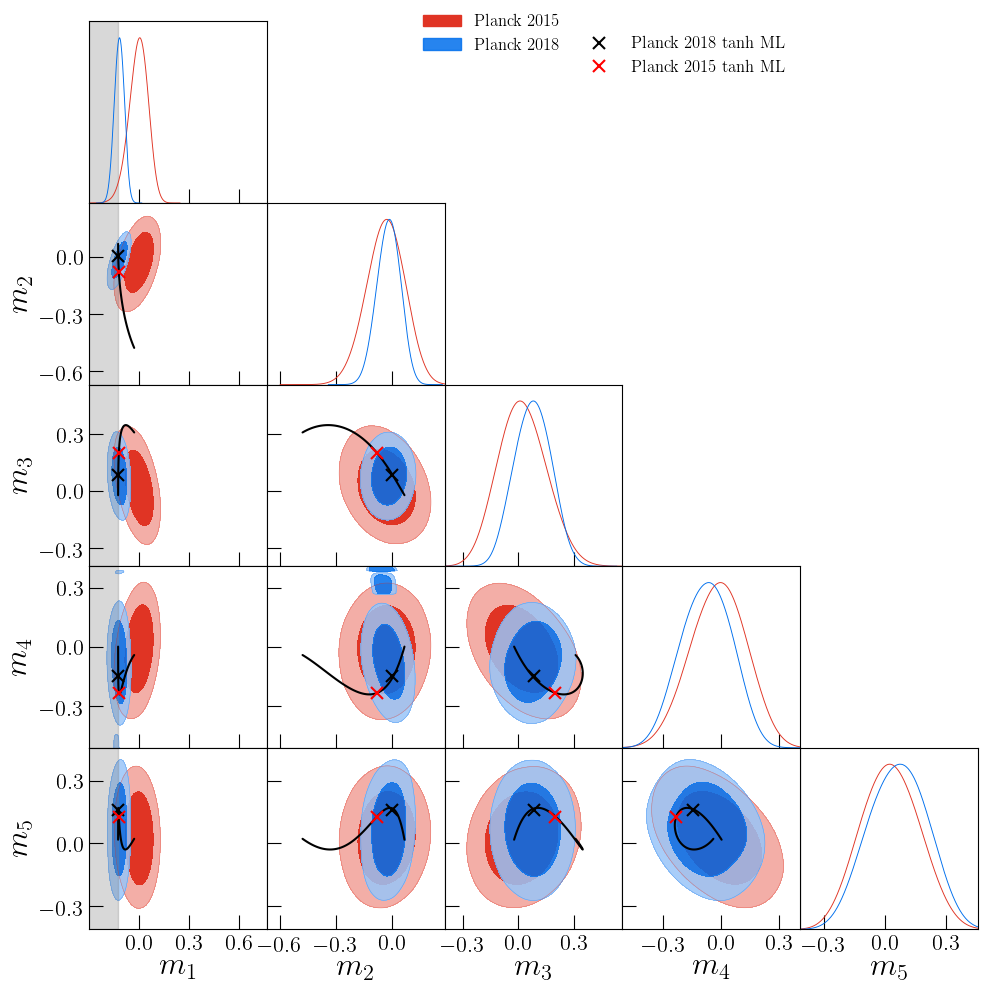
\includegraphics[width=0.7\textwidth]{plots/plot_mj_triangle_t18_r12_t19_t20_vs_pl18_pc_zmax30_pliklite_srollv2_1015_wTauTrajectory_pl15_wTanhML.png}
\caption{Constraints from Planck data on the amplitudes of the five reionization principal components that describe all physical ionization models up to $z_{\rm max} = 30$. We show in red the Planck 2015 and the improved Planck 2018 contours in blue which uses the low-$\ell$ $EE$ likelihood \texttt{srollv2}. The 1D posterior distributions are shown on the diagonal and the 2D 68\% and 95\% C.L. regions in the $m_a-m_b$ planes in the lower triangle. The physicality priors on the ionization history used in this work are delineated by the box boundaries. [TODO: update legend] [Add text: The black solid line indicates the steplike models varying $\tau$. make point that tanh ML is now within the the center of PC constraints]}
\label{fig:plot_mjs_2018_vs_2015}
\end{figure*}
%results/pc_results/plot_mj_triangle_t18_r12_t19_t20_vs_pl18_pc_zmax30_pliklite.pdf
%
In Fig.~\ref{fig:plot_mjs_2018_vs_2015}, we show the 1D posterior and 2D 68\% and 95\% confidence level contours for the 5 PC amplitudes that describe ionization models up to $\zmax=30$. The box boundaries correspond to the physicality priors shown in Eq.~\ref{eq:individualprior} and include all physical models along with some unphysical models. Results using the Planck 2018 data are shown in blue. While all five PC amplitudes are being constrained by Planck, the first two are particularly well-constrained. Contrary to the Planck 2015 results of Ref.~\cite{Heinrich:2016ojb} shown in red, the 2018 data prefers a much smaller amplitude for the first PC, leading to a reduced optical depth.
The trajectories shown in black lines are the steplike models of instantaneous reionization allowed by the Planck 2015 data with the arrow pointing in the direction of increasing optical depth. Clearly, these steplikes models are only a part of the allowed physical model space. By construction, they miss any high-redshift ionization component by assuming neglibile ionization levels before the transition redshift $z_{\rm re}$. 

\begin{figure}
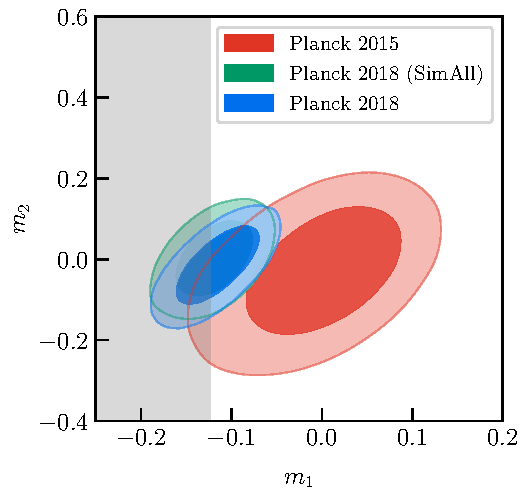
\includegraphics[width=0.40\textwidth]{plots/plot_m1_m2_t18_r12_t19_t20_vs_pl18_pc_zmax30_pliklite_0930_vs_pl18_pc_zmax30_pliklite_srollv2_1015.pdf}
\caption{A zoomed-in of Fig.~\ref{fig:plot_mjs_2018_vs_2015} on the best constrained $\zmax=30$ PC plane, the $m_1-m_2$ plane, comparing Planck 2015 (gray) vs Planck 2018 results using two different low-$\ell$ $EE$ likelihoods: the \texttt{simall\_EE} likelihood (red) vs the \texttt{srollv2} likelihood (blue), the latter had better foreground removal and is the one we show as our fiducial results throughout this paper.
}
\label{fig:plot_m1m2_2015_vs_2018}
\end{figure}

\begin{table}[b]
\centering
\caption{PC chain means $\bar m_a$, standard deviations $\sigma(m_a)$, and correlation matrix $R_{ab}$.}
\label{tab:PC_stats}
\begin{tabular}{|r | r r@{\hskip 0.06in}|r r r r r|}
\hline
		
			  &  \multicolumn{1}{c}{$\bar m_a$} & \multicolumn{1}{c}{$\sigma(m_a)$}	 & \multicolumn{1}{|c}{$m_1$} & \multicolumn{1}{c}{$m_2$} & \multicolumn{1}{c}{$m_3$} & \multicolumn{1}{c}{$m_4$} & \multicolumn{1}{c|}{$m_5$} 
		\\ \hline
		

$m_1$ & -0.119 & -0.098 & 1.000 & 0.657 & 0.208 & 0.094 & 0.067 \\ 
$m_2$ & -0.013 & 0.010 & 0.657 & 1.000 & -0.048 & 0.273 & 0.142 \\ 
$m_3$ & -0.115 & -0.065 & 0.208 & -0.048 & 1.000 & 0.064 & 0.018 \\ 
$m_4$ & -0.025 & 0.085  & 0.094 & 0.273 & 0.064 & 1.000 & 0.195 \\ 
$m_5$ & 0.118 & 0.072  & 0.067 & 0.142 & 0.018 & 0.195 & 1.000 \\ 

\hline
\end{tabular}
\end{table}

\begin{table}[b]
\centering
\caption{Planck 2015 results (with Mortonson PCs) [Will not be in the paper, just for us to compare] }
\label{tab:PC_stats}
\begin{tabular}{|r | r r@{\hskip 0.06in}|r r r r r|}
\hline
		
			  &  \multicolumn{1}{c}{$\bar m_a$} & \multicolumn{1}{c}{$\sigma(m_a)$}	 & \multicolumn{1}{|c}{$m_1$} & \multicolumn{1}{c}{$m_2$} & \multicolumn{1}{c}{$m_3$} & \multicolumn{1}{c}{$m_4$} & \multicolumn{1}{c|}{$m_5$} 
		\\ \hline

$m_1$ 
	& 0.002 & 0.053 & 1.000 & 0.450 & $-$0.432 & 0.273 & $-$0.073 \\ 
$m_2$ 
	& $-$0.030 &  0.101 & 0.450 & 1.000 & $-$0.262 & 0.055 & 0.072 \\ 
$m_3$ 
	& 0.019 &  0.128 & $-$0.432 & $-$0.262 &1.000 & $-$0.417 & 0.155 \\
$m_4$  
	& $-$0.012 & 0.143 &  0.273 & 0.055 & $-$0.417 & 1.000 & $-$0.428 \\ 
$m_5$ 
	& 0.026 & 0.143 & $-$0.073 & 0.072 & 0.155 & $-$0.428 & 1.000\\ 
\hline
\end{tabular}
\end{table}


We show a zoomed version of the $m_1-m_2$ plane in Fig.~\ref{fig:plot_m1m2_2015_vs_2018}, where we show beyond the physicality prior with the shaded area. [Discuss how the ellipse moved in the direction of lower tanh by going to lower m1.] 
In Fig.~\ref{fig:plot_m1m2_2015_vs_2018}, we also show using the PC chain covariance $\bf C$ (black dashed lines) what corresponds to an even simpler effective likelihood, which approximates the $m_a$ posterior as a multivariate Gaussian with mean $\bar{\bf m}$ and covariance $\bf C$ (also shown in Table~\ref{tab:PC_stats}:
\begin{equation}
 {\cal L}_{\rm gauss}\left({\rm data}|\mathbf{m} \right) = \frac{ e^{-\frac{1}{2} ({\bf m}-\bar{\bf m})^T {\bf C}^{-1} ({\bf m}-\bar{\bf m}) } }{\sqrt{(2\pi)^{N_{\rm PC}} | \mathbf{C}| }}.
 \label{eq:gaussian}
 \end{equation}
 This Gaussian approximation agrees well with the actual PC constraints, unlike in the Planck 2015 data where some differences were still visible on top of good agreement. The Gaussian likelihood is even faster than the kernel density estimate, and may be used to sample well-constrained models near the peak of the PC distributions, while becoming possibly less accurate near the tails of the distributions.

In Fig.~\ref{fig:plot_m1m2_lowE_vs_srollv2} we also compare the Planck 2018 results with two different low-$\ell$ $EE$ likelihoods: \texttt{simall\_EE} and \texttt{srollv2}. The \texttt{srollv2} contours are shrunk nearly directly along the lines of constant optical depth $\tau$ ($\tau_{12} = \tau_1 m_1 + \tau_2 m_2$) [wanna show this]? \wh{we might make this point in the context of Marius - that $\tau$ is mainly a linear function of $m_1$, $m_2$, and hence flat priors in $m's$ are locally flat in $\tau$}  [Might be nice to overlay the tanh trajectories, no 1 sigma, 2 sigma business]. 

\wh{I wonder if the order should be reversed and talk about the model testing and KDE first, then the model independent cumulative optical depth?  That way the model stuff could all be introduced here and simulaneously compared with the fiducal results?  The flow could be that we first show more high z optical depth is allowed in the two step model but not FlexKnot and then talk about it being a model independent PC result, concluding that we are more robust than FlexKnot?  Of course I'm assuming that the 2 step model shows this...}

\subsection{Implications for optical depth}

We continue the comparison in the space of cumulative optical depth $\tau(z, \zmax)$, which is a better quantity for visualizing and comparing PC results than the ionization history $x_e$ itself because of it is the quantity most closely related to observables. Recall that these truncated PCs provide only accurate descriptions of the models in terms of their \textit{observable} impact, and are not tools for reconstructing the precise ionization history.

In Fig.~\ref{fig:plot_taugtz_2015_vs_2018}, we compare the 68\% and 95\% confidence level contours in $\tau(z, \zmax)$ for the Planck 2015 (red regions) and the Planck 2018 results (solid lines).
...

In Fig.~\ref{fig:plot_taugtz_lowE_vs_srollv2}, we compare the Planck 2018 results with the two different low-$\ell$ $EE$ likelihoods. [Do we need this?]

In Fig.~\ref{fig:plot_taugtz_PC_vs_tanh}, we compare the PC results against the steplike model. It is clear that the tanh model does not allow for high redshift ionization by construction. The total optical depth allowed by the PC chains sampling the entire physical model space is actually slightly higher due to the contributions from these higher redshifts. [do we want PC version with the physicality priors actually?]\\

We show however, using a separate PC chains with $\zmax = 50$, that there is no evidence for optical depth at higher redshifts than 30. In Fig.~\ref{fig:plot_taugtz_zmax30_vs_zmax50}, we show that the contours in $\tau(z, \zmax)$ are consistent between the $\zmax = 30$ (red regions) and $\zmax = 50$ results (black lines), and that their total optical depth constraints are practically identical: 
\beq
\tau_{\rm PC,\, \zmax=30} = 0.0619^{+0.0056}_{-0.0068}\;\; (\textsc{srollv2}),
\eeq
and
\beq
\tau_{\rm PC,\, \zmax=50} = 0.0626^{+0.0061}_{-0.0072}\;\; (\textsc{srollv2}).
\eeq
These total optical depth constraints have slightly higher central values and smaller error bars compared to those obtained using the original Planck-released \textsc{lowE} likelihood
\beq
\tau_{\rm PC,\, \zmax=30} = 0.0582 ^{+0.0072}_{-0.0083}\;\; (\textsc{lowE}),
\eeq
and
\beq
\tau_{\rm PC,\, \zmax=50} = 0.0582^{+0.0077}_{-0.0088}\;\; (\textsc{lowE}).
\eeq
[more comments here]
%

The upper limit on $\tau(15, \zmax)$ are 
\beq
\tau(15, \zmax)_{\rm PC,\, \zmax=30} < 0.023 \; (95\%\; \mathrm{C.L.})\;\;(\textsc{srollv2}),
\eeq
[double check on full chain (1015) this is from 0930]
and 
\beq
\tau(15, \zmax)_{\rm PC,\, \zmax=50} < 0.022 \; (95\%\; \mathrm{C.L.})\;\;(\textsc{srollv2}).
\eeq

\begin{figure}[ht]
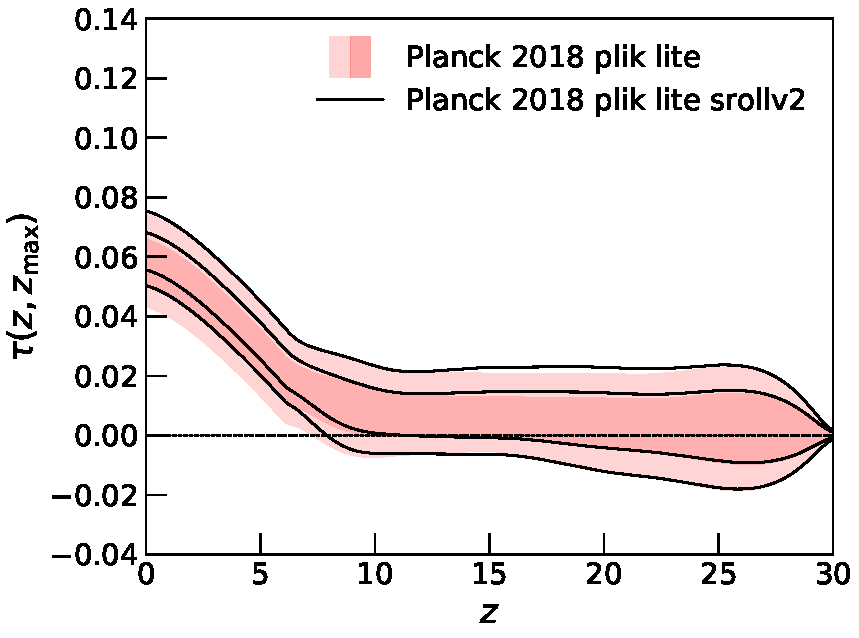
\includegraphics[width=0.45\textwidth]{results/direct_mcmc/pl18_plots_zmax30/plot_pub_tau_gtz_dz_0p1_pl18_pc_zmax30_pliklite_post_0930_and_pl18_pc_zmax30_pliklite_srollv2_0930.pdf}
\caption{[placeholder] PC chains for zmax = 30. Planck 2018 srollv2 likelihood vs Planck 2015).
}
\label{fig:plot_taugtz_2015_vs_2018}
\end{figure}

\begin{figure}[ht]
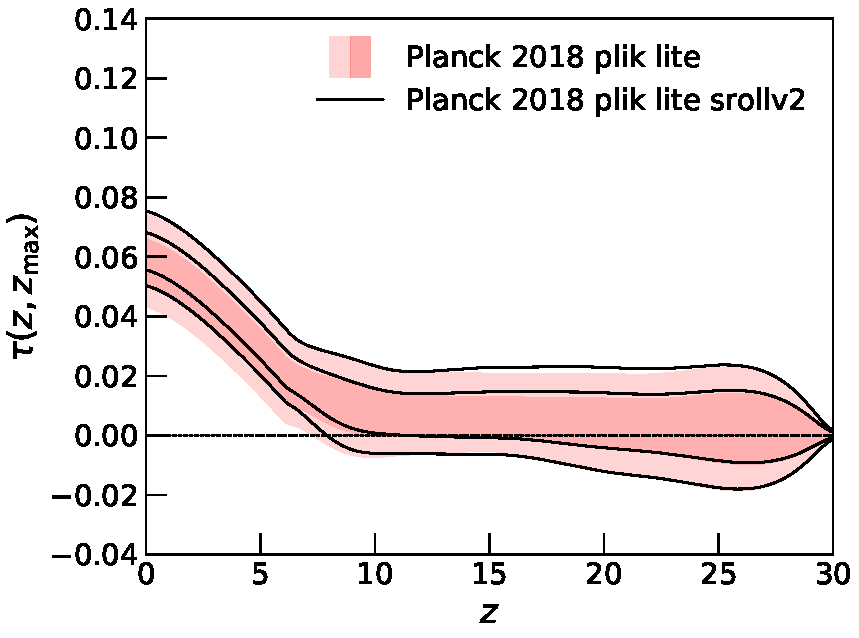
\includegraphics[width=0.45\textwidth]{results/direct_mcmc/pl18_plots_zmax30/plot_pub_tau_gtz_dz_0p1_pl18_pc_zmax30_pliklite_post_0930_and_pl18_pc_zmax30_pliklite_srollv2_0930.pdf}
\caption{PC chains for zmax = 30. Planck 2018 original lowE vs srollv2 likelihood (plik\_lite\_TTTEEE + lowl + simall\_EE vs plik\_lite\_TTTEEE + lowl + sroll2\_EE).
}
\label{fig:plot_taugtz_lowE_vs_srollv2}
\end{figure}


\begin{figure}[ht]
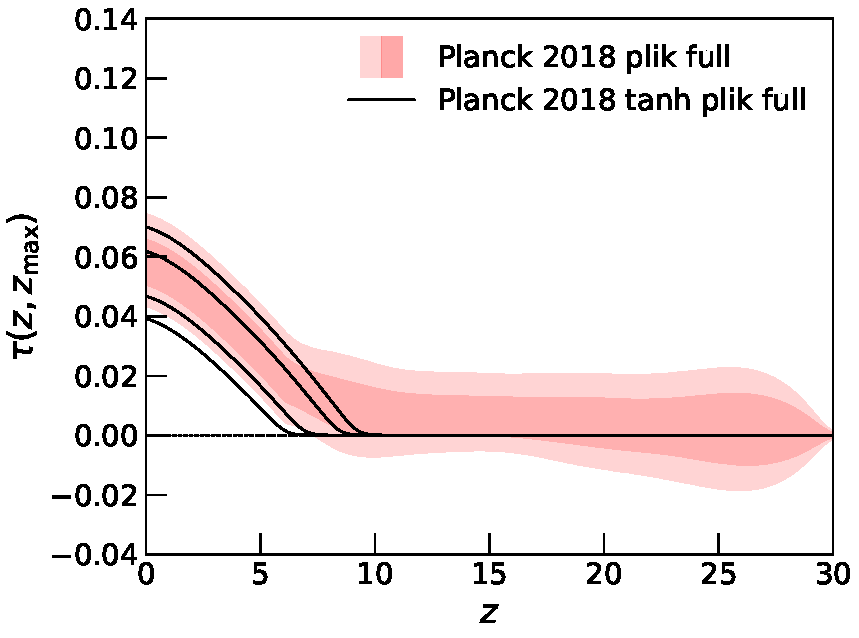
\includegraphics[width=0.5\textwidth]{results/direct_mcmc/pl18_plots_zmax30/plot_pub_tau_gtz_dz_0p1_pl18_pc_zmax30_plikfull_and_pl18_tanh_post_plikfull.pdf}
\caption{PC zmax = 30 vs tanh chains with plik\_full\_TTTEEE for the high-l likelihood.
}
\label{fig:plot_taugtz_PC_vs_tanh}
\end{figure}

\begin{figure}[ht]
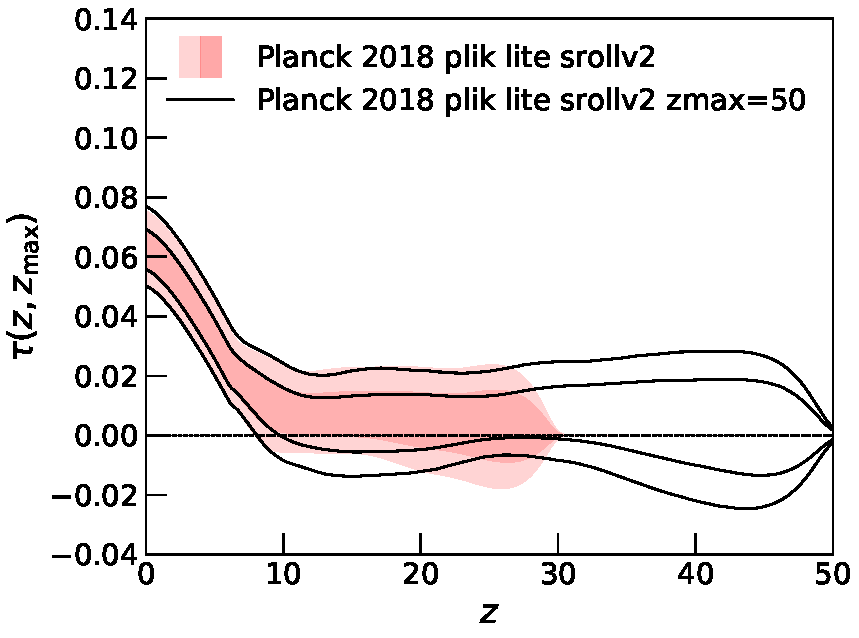
\includegraphics[width=0.45\textwidth]{results/direct_mcmc/pl18_plots_zmax30/plot_pub_tau_gtz_dz_0p1_pl18_pc_zmax30_pliklite_srollv2_0930_and_pl18_pc_zmax50_pliklite_srollv2.pdf}
\caption{Comparing zmax = 30 and 50 PC chains using Planck 2018 original lowE likelihood (plik\_lite\_TTTEEE + lowl + sroll2\_EE). Note that the zmax = 30 uses 5 PCs, whereas the zmax = 50 chains uses 7 PCs. .
}
\label{fig:plot_taugtz_zmax30_vs_zmax50}
\end{figure}


\subsection{Comparison with Previous Results}

The Planck collaboration has released constraints on the total optical depth $\tau$ with a steplike model parameterized by the tanh function, which has evolved from $\tau = 0.067 \pm 0.022$ (Planck 2015) to $\tau = 0.055 \pm 0.009$ (Planck 2016), then to $\tau = 0.0506 \pm 0.0086$ (Planck 2018) [cite papers]. The major improvement comes from clean-up of systematics in the High Frequency Instrument (HFI) data. 

In Planck 2018 VI, using only lowE data and fixing all cosmological parameters including $A_s e^{-2\tau}$, the optical depth constraints was found to be $\tau = 0.0519^{+0.0030}_{-0.0079}$ for a steplike model, $\tau = 0.0504^{+0.0050}
_{-0.0079}$ for the FlexKnot method and $\tau = 0.0487^{+0.0038}_{−0.0081}$ for the PC method with a different prior than that used in this paper. 

They also found the upper limit on high-redshift optical depth to be: $\tau(15, 30) < 0.006$ for the FlexKnot method with a flat $\tau(15, 30)$ prior or $<0.007$ with a flat knot prior. The PC result for the upper limit was not computed. 

Here we show that we find a less stringent upper limit using the PC method $\tau(15, \zmax)_{\rm PC,\, \zmax=30} < XX \; (95\% \mathrm{CL})$. [explain why FlexKnot could give more stringent results.]

\subsection{A note on priors}

In Ref.~\cite{Millea:2018bko} (hereafter MB18)  a concern was raised that the physicality prior we take for the PC analysis in Ref.~\cite{Heinrich:2016ojb} implies a non-flat prior in $\tau$ and introduces bias to the PC result. The authors also proposed a method to flatten the $\tau$ prior by multiplying its inverse at each point in the multidimensional PC space. They claim that adopting the physicality prior used here and in Ref.~\cite{Heinrich:2016ojb} contributed to the a large fraction of the shift in the $\tau$ posterior between the steplike and PC method in the Planck 2015 data. 

In the Planck 2018 paper on cosmological parameters, the reduction of optical depth from the PC results seen in the Planck 2018 data compared to the Planck 2015 data was attributed to the reduction of HFI systematics, with subdominant contribution from priors. We therefore would like to clarify the impacts of the priors we choose and illustrate explicitly that there is no bias with this choice, whereas the flattening method proposed in MB18 is actually at risk of creating a non-flat prior and biasing results.

In the following, we will use $\tau \approx \tau_{12}$ in order to illustrate the impacts of the priors more easily. We first note that by virtue of Eq.~\ref{eq:mmutoxe}, the total optical depth receives contribution from all PCs
\beq
\tau = \tau_{\rm fid} + \sum_a m_a \tau_a,
\eeq
where $\tau_a$ is the contribution from a unit amplitude PC and $\tau_{\rm fid}$, that from the fiducial model. Because most of the contributions to $\tau$ comes from the first two components as shown in Fig. 7 of Ref.~\cite{Heinrich:2018btc} in the appendix, we can approximate it as
\beq
\tau_{12} = \tau_{\rm fid} + m_1 \tau_1 + m_2 \tau_2 \approx \tau.
\eeq
We also show it here in Fig.~\ref{fig:tau12} where the posterior of $\tau_{12}$ and $\tau$ (with five PCs) are compared for the Planck 2018 data.

In Fig.~\ref{fig:prior_box}, we show the Planck 2018 constraints (ellipse) in the $m_1-m_2$ plane along with constant lines of $\tau_{12}$ (light gray). The solid blue box corresponds to the physicality prior, whereas the dashed blue box is constructed to be aligned with the directions of the constant $\tau_{12}$ lines, so that when projected onto the $\tau_{12}$ directions, gives a true flat $\tau_{12}$ prior. The physicality prior upon projection would correspond to a linearly rising prior in $\tau_{12}$ over the region where the posterior has support. One would be eager to conclude that this produces a biased constraint on $\tau_{12}$. However, because the Planck data is more constraining than the prior in $m_1$ and $m_2$, (the ellipse occupying a much smaller area in one part of the prior box), the value of the prior at high $\tau_{12}$ becomes irrelevant for the posterior.

Using the procedure proposed by Ref.~\cite{Millea:2018bko}, inverting the prior value at each point in the PC space, would actually up-weight the high $\tau_{12}$ regions that are not supported by data, while down-weighting the regions that are. This produces an actual bias in the $\tau_{12}$ posterior toward lower optical depth.

We compare the three priors in Fig.~\ref{fig:tau12_posterior_compare_priors} by showing their corresponding $\tau_{12}$ posteriors. Compared to the explicitly flat prior (dashed box in Fig.~\ref{fig:prior_box}) as the ground truth, the posterior from using the physicality prior shifts negligibly. The main difference is a slightly reduced posterior values at very low $\tau_{12}$, which is due to the physicality condition and the restriction that hydrogen reionization be completed by $z = 6$. This is manifested as the data constraint ellipses being partially outside of the solid prior box in Fig.~\ref{fig:prior_box}. A similar effect would be observed for the steplike models with or without the  restrictions that reionization occurs at $z>6$. We also show that the results between the two priors are similar for the $\tau(15, \zmax)$ statistics: $\tau_{12}(15, \zmax) > XX $(95\% C.L.) for the flat $\tau_{12}$ prior vs $\tau_{12}(15, \zmax) > XX $ (95\% C.L.) for the physicality prior.

This is a small difference in comparison to the bias introduced by multiplying the posterior with the inverse of the $\tau_{12}$ prior. [show in figure?] [add a sentence to reiterate that the shift between PC and steplike model seen in the Planck 2015 is not due to the use of physicality prior]. Furthermore, the bias caused by using the inverse prior method in the Planck 2018 data is on the order of $\Delta \tau \sim 10^{-X}$, which could partially [or fully] account for the difference between FlexKnots and PC results seen in Ref.~\cite{Aghanim:2018eyx} on the total optical depth. 

[Discussion of why FlexKnots is too stringent for $\tau_{12}(15, \zmax)$. Not sure how to do yet. Where should this go? Maybe not prior related.]

We conclude that the prior inversion procedure proposed in Ref.~\cite{Millea:2018bko} should not be used where data is more constraining than prior, which includes the Planck 2015, Planck 2018 and possible future datasets.  

 \begin{figure}
          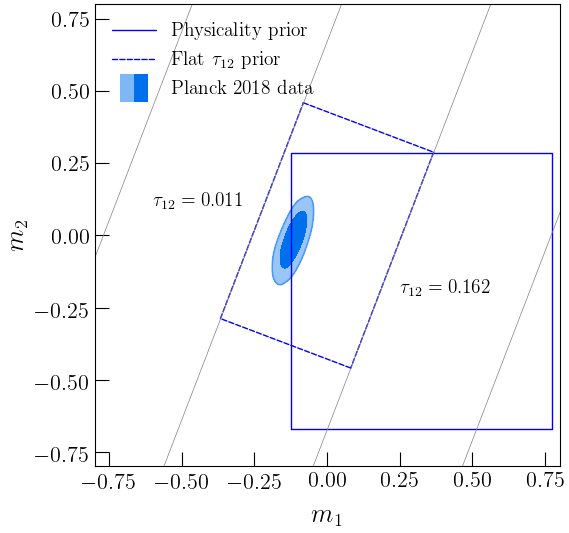
\includegraphics[width=0.9\columnwidth]{paper/plots/pl18_pc_zmax30_pliklite_srollv2_plot_rotated_box_flat_tau_prior_fac_0.8.png}
          \caption {Priors on the $m_1-m_2$ parameter space: the physicality prior (inset square, solid lines) and a flat prior in
          both $\tau_{12}$ and $m_1-m_2$ (rotated rectangle, dashed lines) which are aligned with lines of constant $\tau_{12}$ (light gray lines). Note that although the physicality prior allows for more parameter space at higher $\tau_{12}$, that is also the region excluded by the data constraints (ellipses). The only difference in the allowed region is that the physicality prior clips the low $m_1$ portion of the allowed region due to the physicality condition and the assumption that reionization occurs at $z\ge 6$.} 
          \label{fig:prior_box}
\end{figure}

% NEXT:

% - fill in all numbers: tau(15, 30) upper bounds, store in table or spreadsheet in git; covariance matrix (store in git too); other numbers mentioned in the paper.

% - talk w/ Wayne, finalize decisions, and make polished plots as needed. 

% - write abstract, find title and give the text another pass to refine.

%%%%%%%%%%%%%%%%%%%%%%%%%%%%%%%%%%%%%%%%%%%%

\section{Effective Likelihood}
\label{sec:effective_likelihood}

As described in ~\refsec{KDE}, we turn the PC constraints from the Planck 2018 into an effective likelihood code to constrain arbitrary models of ionization history between $6 \leq z \leq \zmax$. This code is downloadable on Github at \url{} [give URL]. The initial release is offered for the Planck 2018 $\textsc{plik\_lite\_ TTTTTE} + \textsc{lowl} + \textsc{srollv2}$ likelihood combination with $\zmax = 30$. 

To obtain posteriors of model parameters from the corresponding Planck likelihoods, simply specify the functional form for $x_e(z)$ in the code, and run a MCMC analysis using the extension we provide to a MCMC sampler (currently supporting CosmoMC). Note that the likelihood cannot distinguish the effects of the model parameters that impact $z \sim 6$, where the Universe is assumed to be fully ionized. Furthermore, transitions faster than $\Delta z \sim 0.1$ between $6 < z < 6.25$ may not be fully captured because of how PC functions are discretized with $\delta z = 0.25$ and are linearly interpolated within this bin size. [review this statement] To avoid over-smoothing parameter posteriors while maintaining accuracy during the KDE operation, we suggest using the default value of $f = 0.14$. Finally, you may choose to run the chains at a different cosmological model than that of the default Planck 2018 best-fit model, provided it is close enough. 

We demonstrate successful recovery of parameter posteriors using the effective likelihood code by comparing them to a direct MCMC analysis for two examples: 1) The tanh model, which is the standard approach used in CAMB; 2) a two-step toy model which has an one additional parameter to model the high-$z$ ionization as a plateau in $x_e$ before the transition to full ionization happens in the standard tanh model.

\subsection{Example 1: tanh model}
\label{sec:example1}

\begin{figure}
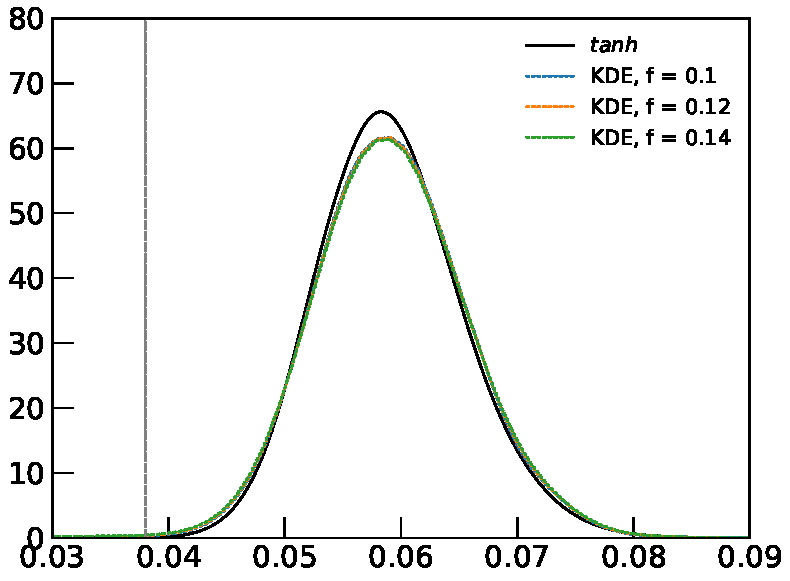
\includegraphics[width=0.40\textwidth]{plots/pl18_pc_zmax30_pliklite_srollv2_1015_tau_posterior_fraccov_1p0_burnin_10000_yes_norm_gaussian0p1_0p12_0p14.pdf}
\caption{Posterior of total optical depth $\tau$: full likelihood (solid) vs effective likelihood (dotted) with f = 0.14 [remove more curves?]. The results agree well; the effective likelihood gives a slightly broader posterior because the kernel density estimate in the PC space introduces smoothing at roughly $\sim$7\% level in the parameter posterior corresponding to $f = 0.14$.
}
\label{fig:tanh_}
\end{figure}

The steplike model used as the standard approach in CAMB describes the hydrogen and singly ionized helium reionization as a tanh function:

 \begin{equation}
x_e(z) = \frac{1+f_{\rm He}}{2}\left\{  1+ \tanh\left[ \frac{y(z_{\rm re})-y(z)}{\Delta y} \right] \right\} + x_e^{\rm rec},
 \label{eqn:tanh_1D}
 \end{equation}
 
 with $y(z)=(1+z)^{3/2}$, $\Delta y=(3/2)(1+z)^{1/2}\Delta z$, and $\Delta z = 0.5$. Here $x_e^{\rm rec}$ is the ionization history from recombination only; the helium fraction
 \beq
 f_{\rm He} = \frac{n_{\rm He}}{n_{H}} = \frac{m_{\rm H}}{m_{\rm He}} \frac{Y_p}{1 - Y_p}, 
 \eeq
 is the ratio of the helium to hydrogen number density, where $Y_p$ is the helium mass fraction, chosen to be consistent with big bang nucleosynthesis for a given baryon density. In addition, the doubly ionized helium reionization is parameterized by an additional tanh function in redshift centered at $z_{\rm He} = 3.5$ with width $\Delta z = 0.5$.

In \reffig{tanh_1D} we show the posterior distribution of the $\tau$ for the effective likelihood results, in which the only sampled parameter is $\tau$ (all other cosmological parameters are fixed at the Planck best-fit model), vs the full likelihood results in which all six $\Lambda$CDM parameters were varied including $\tau$. The posteriors agree well; the effective likelihood gives a slightly broader posterior because the kernel density estimate in the PC space introduces smoothing. We expect the smoothing to be at roughly the $\sim$7\% level in the parameter posterior corresponding to a smoothing factor of $1+f = 1.14$ applied to the covariance of the PCs used for smoothing kernel during KDE.

\begin{itemize}
    \item (here?) Make a point that dz = 0.5 for tanh may not be sufficient for experiments after Planck. This was for higher tau, so transition happens at higher redshift. Now tau is much lower.
    \item{Might also want to address this statement in Planck 2018 paper: ``The TANH result gives slightly higher optical  depth  than  the  others,  which  is  primarily driven  by  the  fixed  duration  of  reionization assumed.” Is this true? Then transition to the following point}
\end{itemize}


 %We take here $z_{\rm re}= 9.85$, corresponding the chain maximum likelihood (ML) model ($\tau = 0.0765$) from \S \ref{sec:MCMC},  for illustrative purposes.   Projected onto 5 PCs and resummed into $x_e(z)$, Eq.~(\ref{eq:mmutoxe}) yields a poor reconstruction of the ionization history itself.
 %Nonetheless as we shall see in Fig.~\ref{fig:clee}, the PC decomposition provides an excellent representation of the polarization power spectrum.
 

\subsection{Example 2: high-z model}
\label{sec:example2}


\begin{figure}
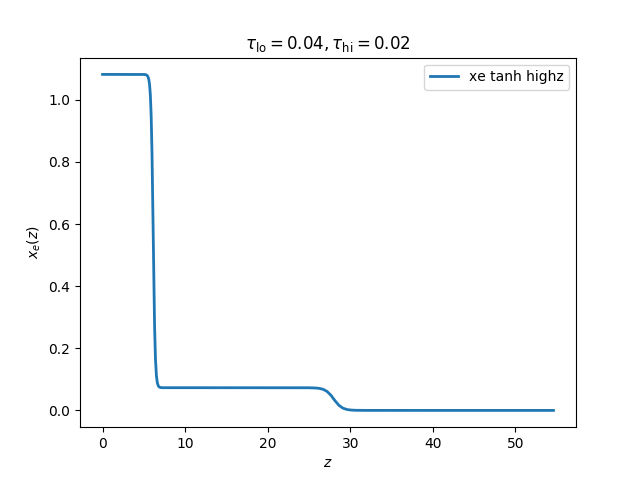
\includegraphics[width=0.5\textwidth]{results/cosmomc_kde/taulo_prior_test/plot_xez_taulo_0p04_tauhi_0p02.png}
\caption{Ionization history $x_e(z)$ of the two-step model $(\taulo, \tauhi) = (0.04, 0.02)$ for the hydrogen and singly ionized helium.
}
\label{fig:two_step_model}
\end{figure}
 
 
The second example is a two-step model, where an additional step is used to give a high-$z$ ionization plateau: 
 \bea
x_e&(z)&\,= \frac{1+f_{\rm He} - \xemin}{2}\left\{  1+ \tanh\left[ \frac{y(z_{\rm re})-y(z)}{\Delta y} \right] \right\} \notag \\
&+& \frac{\xemin - x_e^{\rm rec}}{2}\left\{  1+ \tanh\left[ \frac{z_{\rm t}-z}{\Delta z_{2}} \right] \right\} + x_e^{\rm rec},
 \label{eqn:tanh_highz}
 \eea
where $y(z)=(1+z)^{3/2}$, $\Delta y=(3/2)(1+z)^{1/2}\Delta z_1$ as in the first example, but now we choose $\Delta z_1 = 0.015\, (1+z_{\rm re})$ instead of the usual $\Delta z_1 = 0.5$, to provide sharper distinctions between the two steps.
We choose the second step at $z_{\rm t}=28$ with $\Delta z_2 = 1.0$, since the effective likelihood is limited to models with ionization below $\zmax=30$. 
We recover the standard tanh model in the limit when $\xemin$ approaches the negligible recombination value $x_e^{\rm rec}$.
Therefore this model adds a single parameter $\xemin$ to control the high-$z$ ionization plateau for $z_{\rm re} \lesssim z \lesssim z_t$. We show an example
of this two-step model in Fig.~\ref{fig:two_step_model}.

\begin{figure}[t]
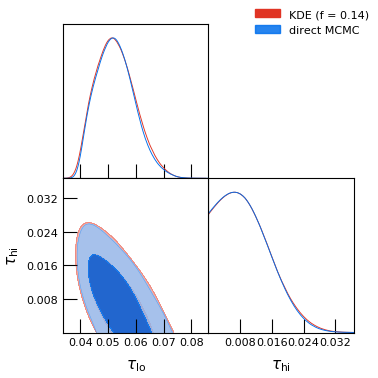
\includegraphics[width=0.47\textwidth]{results/cosmomc_kde/pl18_tanh_highz_test5_run1_vs_relike_tanh_highz_test8_run9_f0p14_taulo_prior_0p03_zre_prior_6p1_taulo_prior_0p0_tri.png}
\caption{Marginalized posteriors for $\tauhi$ and $\taulo$ in the two-step model described in \refssec{example2}: effective reionization likelihood with f = 0.14 (red) agrees very well with the full likelihood results (blue). 
}
\label{fig:two_parameter_model_2D}
\end{figure}

To obtain posterior distributions with flat $\tau$ priors, we convert the model to be parameterized by low and high-redshift optical depth, $\taulo(\zre, \xemin)$ and $\tauhi(\zre, \xemin)$, 
each defined as in Eq.~\refeq{cumtau} but with the boundaries $[0, z_{\rm split}]$ and $[\tau(z_{\rm split}, \infty]$ respectively. We choose the split to be $z_{\rm split} = \zre + \Delta z_2$ to be conservative on the preference of $\tauhi$ in the data. 
We sample in the $(\taulo, \tauhi)$ parameter space and the corresponding ($\zre, \xemin$) is found through an iterative search similar to that used for finding $\zre$ given total $\tau$ in the canonical tanh model. 
The priors are chosen to be $\taulo, \tauhi, \tau_{\rm tot} \in [0, \tau_{\rm max}]$ where $\tau_{\rm max} = 0.35$, and $\tau_{\rm tot} = \taulo + \tauhi$ is the total optical depth for both the effective and full likelihood runs, 
except that we have chosen $\taulo \in [0.03, \tau_{\rm max}]$ for the effective likelihood run. 
Note that $\taulo \lesssim 0.038$ roughly corresponds to $\zre < 6$ in the canonical tanh model. For the two-step model, the correspondence between $\xemin$ and $\zre$ is not one-to-one and depends on the value of $\tauhi$. 
So to make the comparison apples-to-apples, we further apply a prior cut in $\zre$ space to keep models with $\zre > 6.1$ for both the effective reionization likelihood chains and the full likelihood chains.

In ~\reffig{two_parameter_model_2D}, we compare the posteriors of $\taulo$ and $\tauhi$ obtained with these two likelihood codes, which show good agreement. Again we used $f = 0.14$ here for the KDE computation. [add timing results here?] Note that the truncation of the 2D constraint ellipses on the lower end of $\taulo$ is curved cut rather than a straight line, because $\zre$ cut we performed corresponds to a different value of $\taulo$ for a different $\tauhi$. 

The marginalized 1D constraints are $\taulo = XX \pm XX$, $\tauhi = XX \pm XX$ for both runs. The 95\% C.L. upper limit on $\tauhi$ is $\tauhi < XX$ is consistent with the $\tau(15, 30) < XX$ results we got from the PC constraints. [is it? double check] This model of course do not capture the larger space of physical models with high-$z$ ionization like the FlexKnot or PC methods would, but consists of a subset of models for which the high-redshift optical depth results must still be consistent with the constraints from these more general methods. 

To test this, we take the best-fit two-parameter model $(\taulo, \tauhi) = (XX, XX)$ and show its cumulative optical depth $\tau(z, \zmax)$ in ~\reffig{plot_taugtz_two_step_best_fit}. Compared to the PC constraints (shaded regions), this model is within the 95\% upper limit at all redshifts. According to the FlexKnots constraints in Ref.~\cite{}, however, this model would have been ruled out given that $\tau(15, 30) < 0.007$ (95\% C.L.) with the FlexKnots results. [provide comment ...; any further discussion on literature results with FlexKnots?]

[add a conclusive paragraph or sentence]

%Plot: add plot for $\tau(>z)$ contours for the 2 parameter model vs PC; direct integration first?



\begin{figure}[t]
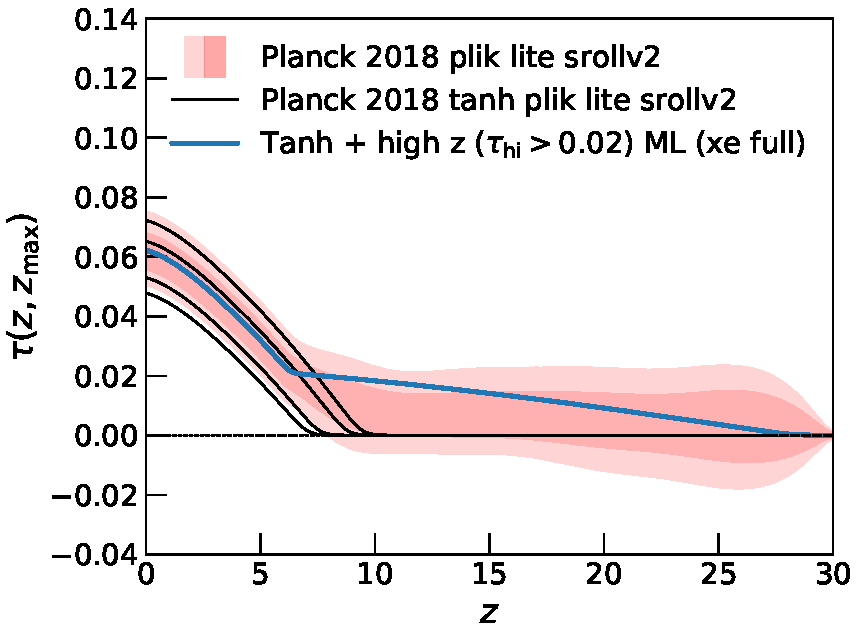
\includegraphics[width=0.450\textwidth]{plots/plot_tau_gtz.pdf}
\caption{Same as \reffig{plot_taugtz_PC_vs_tanh}, but superimposed with the cumulative optical depth $\tau(z, \zmax)$ of the best-fit two-step model. The two-step model is a toy model that adds a high-$z$ ionization plateau to the standard tanh model with one additional parameter. Compared to the cumulative $\tau$ distributions from PCs, the best-fit step-model model is within the 95\% upper limit of the cumulative $\tau$ constraints at all redshifts. 
}
\label{fig:plot_taugtz_two_step_best_fit}
\end{figure}


%\begin{figure}
%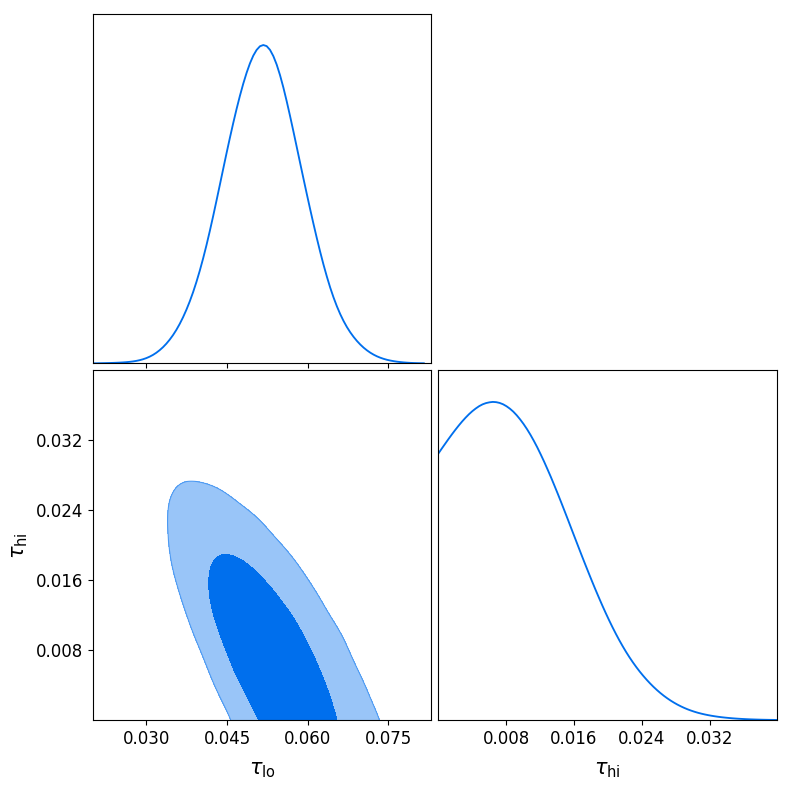
\includegraphics[width=0.5\textwidth]{results/direct_mcmc/two_parameter_model/tauhi_taulo_chains/pl18_tanh_highz_test2_run1_tri.png}
%\caption{Direct MCMC chains of the two-parameter model with \tauhi and \taulo: triangle plot of \tauhi and \taulo. The marginalized 1D constraints are \taulo = $0.0516 \pm 0.0076$, \tauhi = $0.0100 \pm   0.0066$. The ML model is \taulo = 0.0543 and \tauhi = 0.0054 corresponding to $z_{\rm re} = 7.68$ and $x_{e, \mathrm{min}} = 0.021$.
}
%\label{fig:two_parameter_model_2D_plot}
%\end{figure}


%\begin{figure}
%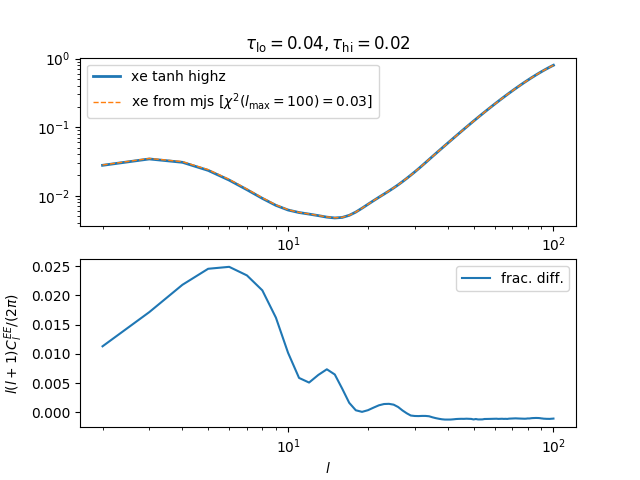
\includegraphics[width=0.5\textwidth]{results/cosmomc_kde/taulo_prior_test/plot_cls_taulo_0p04_tauhi_0p02.png}
%\caption{Testing \taulo prior -- testing that \taulo $\geq$ 0.04 as \taulo prior is OK, by calculating $\chi^2$ between $C_l$ from full $x_e(z)$ vs PC decomposition of the model (\taulo, \tauhi) = (0.04, 0.02). 
%The $\chi^2 = \sum_{2}^{l_{\rm max}} (\Delta C_l^{EE})^2 / \mathrm{Cov}_l = 0.03$ where $\mathrm{Cov}_l = 2 (C_l^{EE})^2/(2l+1)$. } 
%\label{fig:taulo_prior_test_cl}
%\end{figure}

\section{Conclusion}
\label{sec:conclusion}

\begin{itemize}
    \item Summarize what we did in one paragraph.
    \item Give main conclusions in bullet format
    \item main results from PCs: PC constraints, tau, $tau(>z)$.  
    \item comparison w/ Planck 
    \item note on priors
    \item likelihood code, comparisons
    \item other interesting points to discuss and add 
    \item future outlook
\end{itemize}

\bibliography{rei.bib}

\appendix

\section{Outline (in progress)}

\begin{enumerate}
    \item{Intro}
        \begin{enumerate}
            \item 1st paragraph: CMB, reionization, why important
            \item discuss modeling of ionization history in CMB inference, tanh vs PCs (fail to capture high-z; PC captures complete parameter space), mention flex knots/other methods; cite previous PC works.
            \item give context about Planck final results; latest srollv2 likelihood, important to harness all information available, PC allows us to do that and turn into an effective likelihood.
            \item this is what we did: we obtain PC results for Planck 2018, and turn PC chains into a effective likelihood for ionization history: highlight key points like fast inference, entire model space up to zmax 30, code publicly available.
            \item we also compared to Planck official results, which is over stringent at high z, which gives additional motivations for using this likelihood; verified no hint of ionization at z>30; state any additional results.
            \item break down of sections.
        \end{enumerate}

	\item{Background}
		\begin{itemize}
			\item{Reionization Principal Components}	
			\item{Kernel Density Estimate}
		\end{itemize}
	\item{Planck 2018 PC results:\\
		- can discuss discrepancy here on high-redshift tau($>$15) constraints.\\
		- compare with our own 2015 PC results
		- zmax = 30 vs 50}
	\item{Effective Likelihood}
		\begin{itemize}
			\item{Code Description}
			\item{Examples - one and two parameter models}
		\end{itemize}
	\item{Discussion}
		
\end{enumerate}

------ \textbf{Some Numbers} ------ \\

\textbf{Planck official results 2015, 2016, 2018} \\

\begin{itemize}
    
    \item Planck 2015 results (LFI): $\tau = 0.067 \pm 0.022$ (68\%) \\

    \item Planck 2016  intermediate results (LFI): $\tau = 0.055 \pm 0.009$ (68\%) \\
    
    \item Planck 2018 results: $\tau = 0.0506 \pm 0.0086$ (68\%) \\

\end{itemize}

\textbf{Planck 2018 paper} \\

Here lowE means lowE data only, fixing all other cosmological parameters including $A_s e^{-2\tau}$\\

\begin{itemize}

\item $\tau = 0.0519+0.0030-0.0079$ (lowE; flat $\tau$ prior; TANH)(68\%); \\

\item $\tau = 0.0504+0.0050
-0.0079$ (lowE; flat $\tau$ prior; FlexKnot)(68\%); \\

\item $\tau = 0.0487+0.0038
−0.0081$ (lowE; flat $\tau$ prior; PCA)(68\%).

\end{itemize}

\textbf{Upper limit on high-redshift optical depth} (only given for the FlexKnot method):

$\tau(15, 30) < 0.006$ (lowE, flat $\tau(15, 30)$, FlexKnot); \\

$\tau(15, 30) < 0.007$ (lowE, flat knot, FlexKnot).\\

Statements to address:

\begin{enumerate}
    \item {\textbf{Statement on prior in Planck 2018}:  ``Heinrich & Hu (2018) construct a prior that is uniform on τ, but which increases the allowed unphysical parameter space and is chosen a posteriori. Here we instead use the flat prior constructed by the procedure described in Millea & Bouchet (2018) and Handley & Millea (2019), which does not admit extra unphysical models and gives the most generic prior that leaves the prior on $\tau$ uniform."}
    
    \item {Is this statement on tanh in Planck 2018 paper correct?} `` The TANH result gives slightly higher optical depth than the others, which is primarily driven by the fixed duration of reionization assumed."} \\
    
    \item{\textbf{Other comments on our PC prior giving higher optical depth}: ``The PCA result is slightly lower, and is partly affected by the imperfect physicality priors that allow unphysical negative ionization fractions." and ``Millea \& Bouchet showed that the majority of this (2$\sigma$) preference disappeared when using the lower-noise Planck HFI SimLow likelihood (intermediate results reduction of systematics), with an additional sub-dominant effect due to the choice of prior."}
    
\end{enumerate}

How likelihoods and systematics evolved over time:

\begin{enumerate}
    \item 
    \item {Planck 2018 paper attribute the 2018 upper limit on $\tau(15, 30)$ being \textbf{about 3 times more} stringent than the intermediate results by Millea \& Bouchet to the $SimLow \rightarrow SimAll$ where there was better control of systematics in HFI polarization.}
\end{enumerate}


[high redshift going away should be attributed to better control of systematics in HFI polarization data (changes in the SimAll likelihood compared to SimLow) [cite Planck 2018 results cp]]


\end{document}
